\count\Bfootins=1200
\count\Afootins=1200
\count\Cfootins=1200
\pstart
Quod dixi lineam logarithmicam describi motu composito ex aequabili et per detrimentum retardato, ex falso sumseram principio,
componendo duos motus, unum aequabilem, alterum geometricae progressionis.
Cum tamen sit ex vero, verum.
Quia scilicet componendi sunt duo motus, alter aequabilis, alter in applicatis ad hyperbolam,
\edtext{unde logarithmica describitur}{\lemma{unde}\Bfootnote{\textit{(1)}\ fit \textit{(2)}\ logarithmica describitur \textit{L}}} linea.
\pend
\pstart
Nimirum:\edtext{}{\lemma{}\Afootnote{\textit{Am Rand:} NB\vspace{-8mm}}}
si spatia crescunt ut numeri, vires in quolibet spatii puncto existentes decrescunt progressione Geometrica, seu ut potestates.
Ergo contra[,] si vires\protect\index{Sachverzeichnis}{vis} decrescunt ut numeri seu progressione Arithmetica:
spatia percursa\protect\index{Sachverzeichnis}{spatium percursum} erunt ut logarithmi.
Porro in ea ratione qua vires \edtext{crescunt, temporum crementa}{\lemma{crescunt,}\Bfootnote{\textit{(1)}\ tempora \textit{(2)}\ temporum crementa \textit{L}}} decrescunt.
Si vires \edtext{dimidiantur, temporum incrementa duplicantur}{\lemma{dimidiantur,}\Bfootnote{\textit{(1)}\ tempora dupl \textit{(2)}\ tempora qui \textit{(3)}\ temporum [...] duplicantur, \textit{L}}},
nempe spatium \edtext{antea dimidio tempore}{\lemma{antea}\Bfootnote{\textit{(1)}\ duplo te \textit{(2)}\ dimidio tempore \textit{L}}}
percursum, nunc percurretur duplo, sunt scilicet temporum crementa virium crementis reciproca.
Itaque cum reciproca geometrice proportionalium, sint etiam geometrice proportionalia: hinc facile judicari potest;
viribus seu celeritatibus (:~idem enim semper agens unde fit ut hoc loco virium et celeritatum eadem ratio~:) geometrice decrescentibus,
tempora quibus idem aliquod spatium, infinite exiguum percurrendum est geometrice crescere.
Itaque si spatia percursa sint ut numeri, temporum crementa erunt ut potestates seu termini geometricae
\edtext{progressionis; et contra, si temporum crementa}{\lemma{progressionis;}\Bfootnote{\textit{(1)}\ hinc porro sequitur: si spatia \textit{(2)}\ et contra, si  \textit{(a)}\ tempora \textit{(b)}\ temporum crementa \textit{L}}}
sint ut numeri; spatia percursa erunt ut exponentes seu Logarithmi.
Porro quoniam spatiis existentibus ut numeris temporum crementa sunt progressionis geometricae:
ergo spatiis existentibus ut numeris tempora ipsa infinita erunt progressionis Geometricae seu ut potestates,
nam si crementa sint progressionis Geometricae, termini ipsi quorum sunt crementa, erunt etiam progressionis geometricae ipsisque proportionales.
Hinc porro\textso{ si tempora insumta sint ut numeri, spatia percursa erunt ut Logarithmi.}
Quod est Theorema hujus argumenti elegantissimum. Hinc porro sequitur,
spatiorum \edtext{crementa, in quolibet temporis momento}{\lemma{crementa,}\Bfootnote{\textit{(1)}\ iisdem temporibus sumtis \textit{(2)}\ in quolibet [...] momento, \textit{L}}},
procedere ut applicatas hyperbolae, seu esse progressionis Harmonicae quia crementa logarithmorum sunt applicatae hyperbolae ex invento
Gregorii a \edtext{S. Vincentio\protect\index{Namensregister}{\textso{Saint-Vincent}, Gr\'{e}goire de (Gregorius a S. Vincentio) S.J. 1584-1667}.}{\lemma{S. Vincentio}\Cfootnote{\cite{00316}G. \textsc{de Saint-Vincent}, \textit{Opus geometricum}, Antwerpen 1647, l. VI, prop. 129, S. 596f.}}
\pend
%\newpage
%\vspace{4mm}
%\vspace*{2em}
\pstart
   \edtext{Vires ergo sunt in ratione temporum reciproca. Sunt enim vires ut spatiorum incrementa. Ergo retardationes virium erunt, ut differentiae applicatarum hyperbolae, ad asymptoton, seu in ratione temporum reciproca duplicata.}{\lemma{}\Bfootnote{\textit{(1)}\ Si tempora sint ut numeri \textit{(2)}\ Vires ergo [...] duplicata. \textit{erg.} \textit{L}}}
Hinc jam\textso{ ponendo }\edtext{\textso{aliquod corpus}}{\lemma{\textso{aliquod}}\Bfootnote{\textit{(1)}\ \textso{punctum} \textit{(2)}\ \textso{corpus} \textit{L}}}\textso{ moveri in unam partem aequabili motu, in alteram motu per detrimentum retardato,}
ita ut directio unius ad directionem alterius sit perpendicularis, aliumve faciat angulum,
patet eodem momento nunc huc,
\edtext{fig. 1,}{\lemma{}\Bfootnote{fig. 1, \textit{erg.} \textit{L}}}
versus $\displaystyle C$, per rectas aequales $\displaystyle AB$, $\displaystyle BC$, moveri,
nunc illuc versus \edtext{$\displaystyle H$, per [procedentes]}{\lemma{$\displaystyle H$, per}\Bfootnote{%
\textit{(1)}\ crescentes %
\textit{(2)}\ procedentium \textit{L ändert Hrsg.}}}
harmonice, $\displaystyle AD$, $\displaystyle EF$, $\displaystyle GH$, summae autem harmonice crescentium sunt
\edtext{logarithmice procedentes}{\lemma{logarithmice}\Bfootnote{\textit{(1)}\ crescentes \textit{(2)}\ procedentes. \textit{L}}}.
Ergo\textso{ linea curva }$\displaystyle DFH$\textso{ est logarithmica.}
Demonstrari hoc potest etiam non assumpto
\edtext{San-Vincentii theoremate:}{\lemma{San-Vincentii theoremate}\Cfootnote{a.a.O.}}
quia eadem ipsa linea quae spatiorum ad tempora relationes referebat, restituitur
(:~qualiscunque fuerit progressio differentiarum~:) ea autem erat logarithmica.
\pend
\vspace{2.5em}
\pstart 
\begin{minipage}[c]{0.4\textwidth}
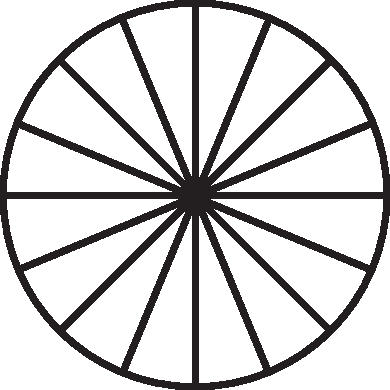
\includegraphics[trim = -25mm -6mm 0mm 0mm, clip, width=0.7\textwidth]{images/lh03705_011v-d1.pdf}
\end{minipage}
\hspace*{13,3mm}
\begin{minipage}[c]{0.6\textwidth}
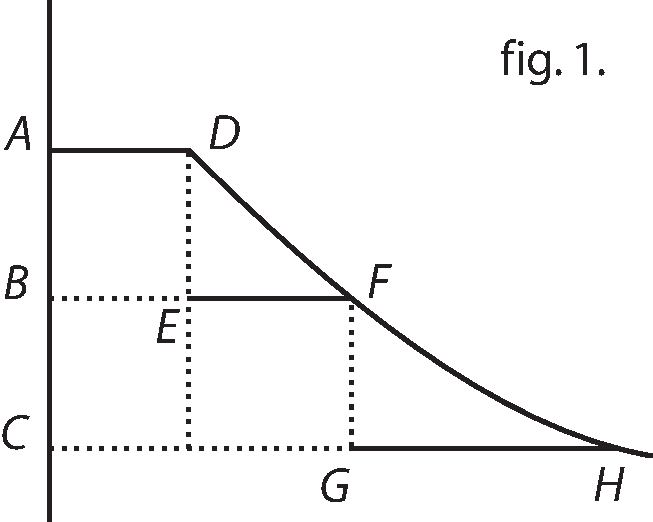
\includegraphics[trim = 0mm -6mm 0mm 0mm, clip, width=0.64\textwidth]{images/lh03705_011v-d2.pdf}
\end{minipage}\\
\hspace*{24mm} [\textit{Fig. 6}]\hspace*{56mm} [\textit{Fig. 7}]
\pend
\newpage
\count\Bfootins=1100
\count\Afootins=1100
\count\Cfootins=1100
\pstart
\noindent
\centering
    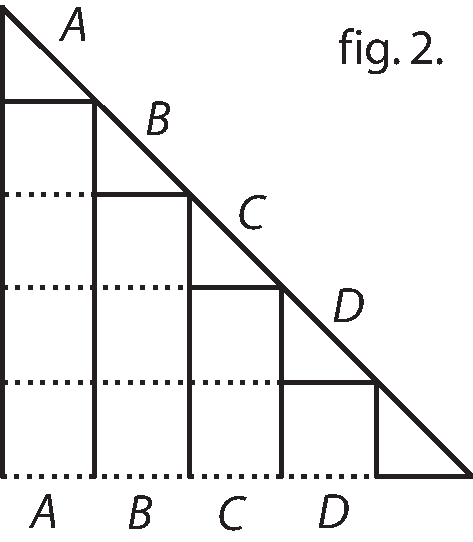
\includegraphics[trim = 0mm -3mm 0mm -3mm, clip,width=0.27\textwidth]{images/lh03705_011v-d3.pdf}
    \pend
    \pstart
    \edtext{}{\lemma{}\killnumber\Afootnote{\textit{Unter} [\textit{Fig. 8}]:\vspace*{4mm}\\
$\displaystyle %\renewcommand{\arraystretch}{1.2} 
\protect\begin{array}{llllll} \frac{a}{1}& b &&&&1\\
\frac{a}{2} & c & b &&&2\\
\frac{a}{3} & d & c & b &&3\\
\frac{a}{4} & e & d & c & b &4\\
\frac{a}{5} & f & e & d & c &5\\ \protect\end{array}$\vspace{-10mm}}}
\noindent \centering
    [\textit{Fig. 8}] % \caption{Bildbeschreibung}
        \pend
        \vspace{1.5em}
\pstart
Invenimus \setline{1}paulo ante, si motus per se sit
\edtext{aequabilis spatia quolibet momento}{\lemma{aequabilis}\Bfootnote{\textit{(1)}\ in quolibet momento spatia ex motu \textit{(2)}\ spatia [...] momento \textit{L}}}
percursa decrescere ut applicatas hyperbolae.
Quid vero si motus per se sit acceleratus?
Fingere possumus compositum ex pluribus aequabilibus,
\edtext{fig. 2,}{\lemma{}\Bfootnote{fig. 2, \textit{erg.} \textit{L}}}
$\displaystyle A.$ $\displaystyle B.$ $\displaystyle C.$ $\displaystyle D.$
ex quibus posito primum retardari ita ut primo momento spatium percursum sit
\edtext{$\displaystyle b$, 2\textsuperscript{do}}{\lemma{$\displaystyle b$,}\Bfootnote{\textit{(1)}\ tertio \textit{(2)}\ 2\textsuperscript{do} \textit{L}}}
\edtext{$\displaystyle c$, 3\textsuperscript{tio}}{\lemma{$\displaystyle c$,}\Bfootnote{\textit{(1)}\ quarto \textit{(2)}\ 3\textsuperscript{tio} \textit{L}}}
$\displaystyle d$, quarto
\edtext{$\displaystyle e$, quinto $\displaystyle f$}{\lemma{$\displaystyle e$,}\Bfootnote{\textit{(1)}\ sexto $\displaystyle g$ \textit{(2)}\ quinto  \textit{L}}}:
alter ita retardabitur, ut secundo momento spatium sit ut $\displaystyle b$, tertio ut $\displaystyle c$, quarto ut $\displaystyle d$, quinto ut $\displaystyle e$
\edtext{etc.}{\lemma{}\Bfootnote{etc. \textit{erg.} \textit{L}}},
nam primo momento cum nondum existat, non retardatur.
Itemque tertius ita retardabitur, ut tertio momento (nam primo et secundo nondum existit) spatium sit ut $\displaystyle b$, quarto ut $\displaystyle c$, quinto ut $\displaystyle d$, etc.
et ita in reliquis.\\
\hspace*{7,5mm}
    Unde patet applicatas, seu spatia quolibet momento
\edtext{percursa, esse ut seriei ipsius summas}{\lemma{percursa,}\Bfootnote{\textit{(1)}\ esse ut in unam partem \textit{(2)}\ esse [...] summas, \textit{L}}},
seu ut logarithmos (:~ubi rursus opus non est nosse naturam differentiae \edtext{logarithmorum~:). Ecce ergo}{\lemma{logarithmorum~:).}\Bfootnote{\textit{(1)}\ Jam spatia percursa ab altera parte \textit{(2)}\ Ecce ergo \textit{L}}}
mirum iterum theorema: In motu per se aequabiliter
accelerato spatiorum quolibet momento percursorum
\edtext{crementa, [sunt] ut logarithmi}{\lemma{crementa,}\Bfootnote{\textit{(1)}\ sunt ut logarithmi \textit{(2)}\ crescunt ut logarithmi \textit{(3)}\ \textbar\ sunt \textit{erg. Hrsg.}\  \textbar \ ut logarithmi, \textit{L}}},
si tempora insumta crescant ut numeri;
itaque si spatiorum crementa ponantur ut numeri,
erunt tempora percursa ut potestates, adeoque et momenta
\edtext{seu temporum}{\lemma{seu}\Bfootnote{\textit{(1)}\ celeritatum \textit{(2)}\ temporum \textit{L}}}
crementa ut potestates.
Ergo\textso{ si temporum crementa ut numeri, erunt spatiorum crementa ut logarithmi in motu aequabiliter per se accelerato, ob detritum retardato.}
Ergo \edtext{si tempora}{\lemma{si}\Bfootnote{\textit{(1)}\ temporum cre \textit{(2)}\ tempora \textit{L}}}
ut quadrati, erunt spatia ut summae logarithmorum a radicibus.
Ergo si tempora ut numeri spatia erunt summae semilogarithmorum, ergo et ut summae logarithmorum.
Nempe si tempora \edtext{insumta}{\lemma{}\Bfootnote{insumta \textit{erg. L}}}
sunt ut \edtext{numeri, spatia percursa sunt}{\lemma{numeri,}\Bfootnote{\textit{(1)}\ spatia sunt \textit{(2)}\ spatia percursa sunt \textit{L}}}
ut logarithmorum summae.
In motu per se aequabiliter accelerato, per detrimentum retardato,
\edtext{ut patet ex dicto paulo ante}{\lemma{ut}\Bfootnote{\textit{(1)}\ ex superioribus \textit{(2)}\ patet [...] ante, \textit{L}}},
\edtext{si vires}{\lemma{si}\Bfootnote{\textit{(1)}\ vires \textit{(2)}\ virium momento \textit{(3)}\ vires \textit{L}}}
sunt progressionis harmonicae (nempe temporum crementis reciprocae quae sunt ut
\edtext{numeri), erunt}{\lemma{}\Bfootnote{numeri),  \textbar\ sive vires ipsae progressionis logarithmicae, \textit{gestr.}\ \textbar\ erunt \textit{L}}}
\edtext{spatia ut summae logarithmorum}{\lemma{spatia ut summae}\Bfootnote{\textit{(1)}\ summarum \textit{(2)}\ logarithmorum \textit{L}}}
seu ut summae \edtext{summarum}{\lemma{}\Bfootnote{summarum \textit{erg. L}}} ipsarum virium.
Ergo\textso{ si vires sint ut numeri, erunt spatia percursa ut cubi.} Atque ita praeter omnem spem ad lineam perventum est Analyticam, quae alia forte via non apparuisset.\hfill
\edtext{Scilicet\hfill mutanda}{\lemma{Scilicet}\Bfootnote{\textit{(1)}\ si \textit{(2)}\ mutanda \textit{L}}}\hfill
est\hfill enuntiatio\hfill ope\hfill summarum,\hfill qua\hfill fit\hfill transitus\hfill a\hfill figuris 
\pend
\vspace{1em}
\pstart
\noindent
\centering
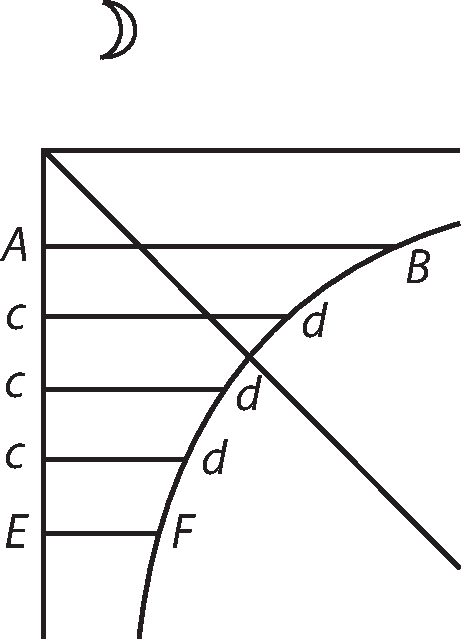
\includegraphics[trim = 0mm -3mm 0mm 0mm, clip, width=0.27\textwidth]{images/lh03705_011v-d4.pdf}\\
\centering
 [\textit{Fig. 9}] % \caption{[\textit{Fig. 9}]}
\pend
\newpage
\pstart \noindent
Analyticis ad Transcendentes apertus
a \edtext{San Vincentio\protect\index{Namensregister}{\textso{Saint-Vincent}, Gr\'{e}goire de (Gregorius a S. Vincentio) S.J. 1584-1667}.}{\lemma{San Vincentio}\Cfootnote{\cite{00316}a.a.O.}}
Nota spatiis crescentibus tempora decrescunt, (quia vires crescunt)
an tamen et temporum crementa crescunt aut decrescunt?
Hoc variat.
\pend
\count\Bfootins=1200
\count\Afootins=1200
\count\Cfootins=1200
\pstart
%\begin{wrapfigure}[13]{l}{0.31\textwidth}
%    \vspace{-4.5mm} 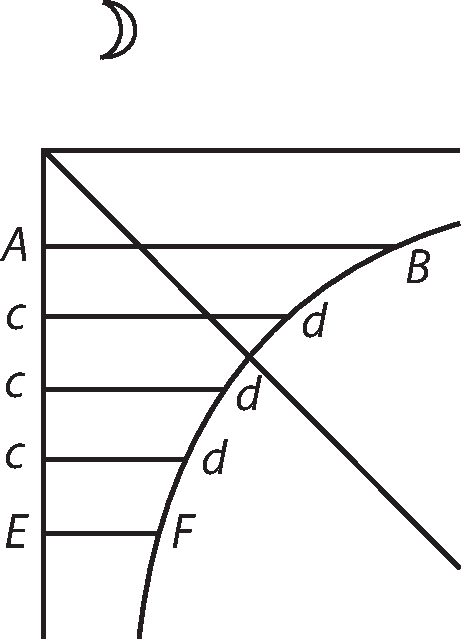
\includegraphics[trim = 0mm -3mm -6mm 0mm, clip, width=0.31\textwidth]{images/lh03705_011v-d4.pdf}
%    \centering
%    [\textit{Fig. 9}] % \caption{[\textit{Fig. 9}]}
%   \end{wrapfigure}
    Videndum tamen an quod dixi de summa summarum sit verum sive crescant sive decrescant spatia, \edtext{tempora aut celeritates,}{\lemma{tempora aut}\Bfootnote{\textit{(1)}\ vires \textit{(2)}\ celeritates, \textit{L}}}
aut horum crementa.
Si curva $\displaystyle BdF$[,] \edtext{fig. $\rightmoon$}{\lemma{}\Bfootnote{fig. $\rightmoon$ \textit{ erg. L}}}\edtext{[,]}{\lemma{fig. $\rightmoon$}\Cfootnote{[\textit{Fig. 9}] nach unserer Zählung.}}  
% PR: $\rightmoon$ ist ein Mondzeichen aus dem LateX-Vorrat
Hyperbola, et $\displaystyle Ac$ sint ut numeri, erunt $\displaystyle BAcdB$ ut
\edtext{Logarithmi. Imo, etiam}{\lemma{Logarithmi.}\Bfootnote{\textit{(1)}\ Etiam \textit{(2)}\ Imo, etiam \textit{L}}}
inverso modo 
sumtis $\displaystyle Ec$ ut numeris, poterunt $\displaystyle FEcdF$ sumi pro logarithmis,
ob rationem allegatam 
   supra, ubi inversos logarithmos, qui substractione unica a quantitate constanti fiunt ex
\edtext{ordinatis, ostendi}{\lemma{}\Bfootnote{ordinatis,  \textbar\ et \textit{gestr.}\ \textbar\ ostendi \textit{L}}}
esse veros, vide \edtext{fig. $\Sun$.}{\lemma{fig. $\Sun$}\Cfootnote{[\textit{Fig. 1}] nach unserer Zählung.}}% PR: $\Sun$ ist ein Sonnenzeichen aus dem LateX-Vorrat
%\pend